%------------------------------------------------------------------------
%Editar Diplomado
\hypertarget{cv:modificarActor}{\section{Modificar Actor}} \label{sec:modificarActor}

	Esta funcionalidad le permitirá modificar la información de un actor previamente registrado con el fin de corregir o actualizar datos del mismo. 

		\subsection{Procedimiento}

			%Pasos de procedimiento
			\begin{enumerate}
	
			\item Oprima el botón \IUEditar{} de algún registro existente de la pantalla \ref{fig:GestionarActores} ''Gestionar Actores''.
	
			\item Se mostrará la pantalla \ref{fig:modificarActor} ''Modificar Actor''.
			
			%Pantalla
			\begin{figure}[htbp!]
				\begin{center}
					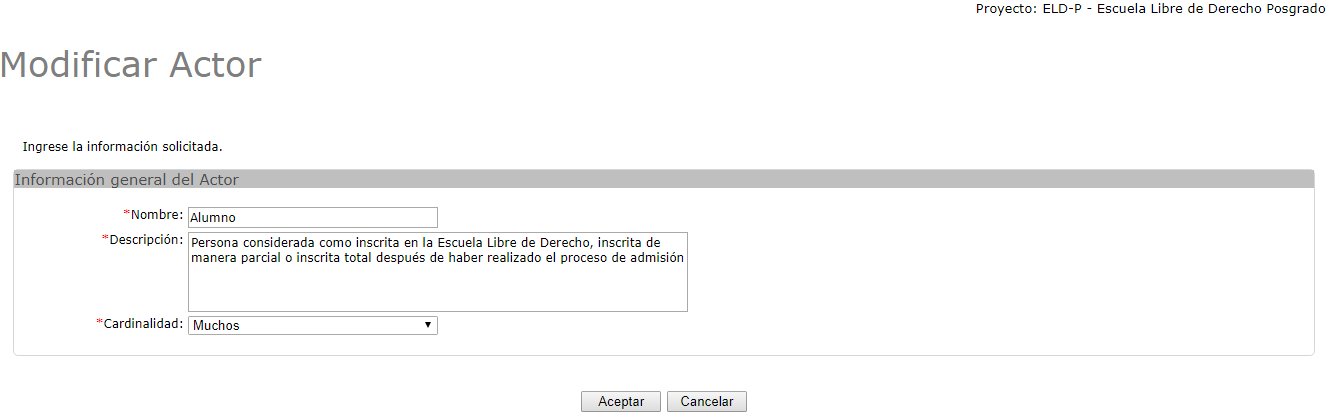
\includegraphics[scale=0.5]{roles/lider/actor/pantallas/IU10-2modificarActor}
					\caption{Modificar Actor}
					\label{fig:modificarActor}
				\end{center}
			\end{figure}
		
			\item Modifique los datos solicitados por la pantalla.
						
			\item Oprima el botón \IUAceptar.
			
			\item Se mostrará el mensaje \ref{fig:actorModificado} en la pantalla \ref{fig:GestionarActores} ''Gestionar Actores''.
			
			\begin{figure}[htbp!]
				\begin{center}
					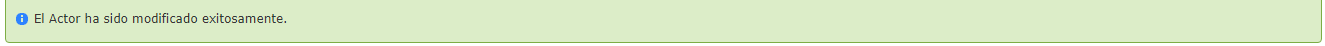
\includegraphics[scale=0.5]{roles/lider/actor/pantallas/IU10-2MSG1}
					\caption{MSG: Actor Actualizado}
					\label{fig:actorModificado}
				\end{center}
			\end{figure}
			\end{enumerate}